
\chapter{On the relationship between Arctic winter precipitation and minimum sea ice extent}
\label{chap:winter_prec}

This chapter is to be submitted to \textit{Geophysical Research Letters}.

\section*{Abstract}

In the past three decades, the Arctic has experienced large declines in summer sea ice cover, permafrost extent and spring snow cover, and increases in winter precipitation.
This study explores the relationship between declining Arctic sea ice extent and early winter precipitation across the high-latitude Arctic land masses.
The first part of this chapter presents the observed relationship between sea ice extent and winter precipitation.
Using satellite estimates of sea ice extent and precipitation data based on a combination of in-situ observations and global reanalyses, we show that early winter precipitation is negatively correlated with summer sea ice extent and that this relationship is strongest before the year 2000.
After 2000, around the time sea ice extent minima began to decline most rapidly, the relationship between sea ice extent and early winter precipitation degenerates.
This indicates that other processes are driving changes in sea ice extent and winter precipitation.
We hypothesize that the observed correlations between sea ice extent and high winter precipitation are related to anomalous patterns in ocean evaporation and sea ice extent in the fall.
To better understand the physical mechanisms driving the observed changes in the Arctic climate system and the sensitivity of the Arctic climate system to declining sea ice, we have used the fully-coupled Regional Arctic System Model (RASM) to simulate two distinct sea ice climates.
The first climate represents normal sea ice extent, while the second and third represent reduced summer sea ice extent.
The second portion of this chapter analyzes these three RASM simulations, in conjunction with our observation-based analysis, to understand the coupled relationship between poleward moisture transport, sea ice extent, evaporation from the Arctic Ocean, and precipitation.
We will present the RASM-simulated Arctic water budget and demonstrate the role of sea ice extent in driving winter precipitation anomalies.
Finally, we use the Self-Organizing Map (SOM) machine learning technique to identify characteristic patterns of ocean evaporation, sea ice extent, and polar cap convergence that contribute to anomalies in early winter precipitation.

\section{Introduction}
\label{sec:intro_ch5}

In the past three decades, the Arctic region has experienced unprecedented changes in key cryospheric processes.
Rapid declines in sea ice cover have been accompanied by reductions permafrost extent and spring snow cover, and increases in winter precipitation and winter snow accumulations \citep{Kohler_2006,Callaghan_2011,Bulygina_2009}.
The combination of these changes has had a marked impact on the regional and global climate systems.
Driving much of these changes has been a regional warming trend that is nearly twice as large as the global mean \citep{Serreze_2006c,Screen_2010}.
This disparity in temperature increases is often referred to as Arctic Amplification and is largely explained by the ice-albedo feedback \citep{Curry_1995}.
While this is likely the primary mechanism encouraging the rapid warming in the Arctic, other secondary feedback processes are also at play.
One such feedback process relates the state and fluxes of the Arctic Ocean (SSTs, sea ice cover, evaporation) to precipitation over land, which modulates winter snow cover and permafrost health.

Observational evidence of an amplified hydrologic cycle \citep{Stocker_2005} has been found in the form of increasing precipitation \citep{Rawlins_2006}, runoff \citep{Peterson_2002}, and winter snow accumulations \citep{Kohler_2006,Bulygina_2009}.
While global average precipitation is expected increase following a muted response to warming via the Clausius-Clapeyron relationship \citep[e.g. ][]{Held_2006,Stephens_2008,Byrne_2015}, precipitation increases in the Arctic are expected exceed the in the global average \citep{Stocker_2005}.
Analysis of the collection Earth system models (ESMs) in the Coupled Model Intercomparison Project Phase 5 \citep[CMIP5; ][]{Taylor_2012} by \citet{Bintanja_2014} indicates that annual precipitation changes in the Arctic may exceed 50\%, with the largest relative increases in the winter over the Arctic Ocean.
\citet{Bintanja_2014} also identify that the majority of these changes are due to precipitation sourced from enhanced local evaporation related to retreating sea ice.
This somewhat contradicts previous work that suggested increased poleward moisture transport was the main driver of Arctic precipitation increases and, combined with the intermodel spread of precipitation changes, brings into question sensitivity of modern ESMs.
Therefore, the precise response of precipitation to decreasing sea ice extent remains somewhat unclear.
ESMs, along with statistical models, tend to poorly represent the observed decline in summer sea ice extent.
This is evidenced by the intermodel spread among the 39 ESMs analyzed by \citet{Bintanja_2014}.
In their study, changes in sea ice extent between the beginning and end of the twenty-first century ranged between 31.2-66.2\%, while changes in precipitation varied by a factor of three to four.

Conceptually, it is relatively easy to reason how a warmer Arctic Ocean with less sea ice will lead to increased surface evaporation, and how this could lead to enhanced divergence of moisture onto land in the form of precipitation.
Because high-latitude land areas are predominantly below freezing in the fall, increases in precipitation during this season are expected to produce deeper snow packs.
This process would then act to further insulate the underlying ground and suppressing the cold season cooling of high-latitude permafrost \citep{Osterkamp_1999,Zhang_2005,Lawrence_2010}.
Further permafrost degradation may be attributed to earlier spring snow melt driven by regional warming and possibly be increased surface infiltration of warm meltwater \citep{Lawrence_2010}.

The question of how the Arctic climate will respond to such large temperature and sea ice changes has been at the forefront of recent scientific research \citep[e.g. ][]{Kazutoshi_2014,Simmonds_2014,Wegmann_2015,Vihma_2014}.
Here, we investigate the relationship between Arctic winter precipitation, ocean evaporation, and sea ice extent to better understand the terrestrial precipitation response to the ongoing sea ice decline.
Our apriori hypothesis is that the reductions in sea ice extent in would lead to increases in evaporation from the central portions of the Arctic Ocean and precipitation over land during the fall and early winter months.
We test this hypothesis using three simulations spanning a range of sea ice climates from from a fully-coupled regional climate model described in Section \ref{sec:data_models_ch5}.
In Section \ref{sec:results_ch5} we present our analysis of these simulations, first computing the regional freshwater budget following \citet{Serreze_2006a}, then using the Self-Organizing Map (SOM) machine learning technique for dimension reduction and pattern evaluation \citep{Kohonen_1998,Hewitson_2002}.

\section{Data and Methods}
\label{sec:data_models_ch5}

We utilize three simulations from the Regional Arctic System Model \citep[RASM; ][]{Hamman_2016a,Roberts_2015a}.
RASM is a high-resolution fully-coupled regional ESM that has been recently developed to improve the representation of coupled Arctic processes.
\citet{Hamman_2016b} provide a complete description of the configuration of RASM for the baseline $RASM_{CONTROL}$ simulation.
Two sensitivity simulations, $RASM_{RSI}$ and $RASM_{RSH}$, representing intermediate and high reductions in sea ice extent are also utilized.
The configuration of simulations are identical to $RASM_{CONTROL}$ except in the parameterization of sea ice albedos, which is summarized in Table \ref{table:sims}.
RASM is forced at its lateral boundaries with the ERA-Interim Reanalysis \citep{Dee_2011}.
It is important to note that spectral nudging is applied to temperature and winds in RASM above 500 hPa \citep{Cassano_2016}.
From a practical perspective, this nudging means that the synoptic scale circulation patterns in all three RASM simulations closely match those of ERA-Interim \citep{Glisan_2013}.

\begin{table}[]
    \centering
    \caption{Summary of RASM simulations used in this chapter.}
    \label{table:sims}
    \begin{tabular}{|l|p{4in}|}
    \hline
    \textbf{Dataset} & \textbf{Sea Ice / Ocean Configuration}                                                                                                         \\ \hline
    $RASM_{CONTROL}$    & Default RASM (see \citet{Hamman_2016b})                                                                                                          \\ \hline
    $RASM_{RSI}$         & \begin{tabular}[c]{@{}l@{}}Ocean: No changes\\ Sea Ice: Snow albedo -0.5 std. dev. of observed.\end{tabular}                                   \\ \hline
    $RASM_{RSH}$         & \begin{tabular}[c]{@{}p{3.5in}}Ocean: No changes\\ Sea Ice: No sea ice initial condition, reduced snow/ice/pond albedo -2.0 std. dev.
    \end{tabular} \\ \hline
    \end{tabular}
\end{table}

Observations of sea ice extent are taken from the National Snow and Ice Data Center Weekly Sea Ice Extent product \citep{Brodzik_2013}.
Gridded precipitations observations between 1979 and 2014 are taken from CRU TS v. 3.23 \citep{Harris_2014}.
% TODO: reference reanalyses

\section{Results and Discussion}
\label{sec:results_ch5}
\subsection{Observational evidence}

\begin{figure}
  \centering
  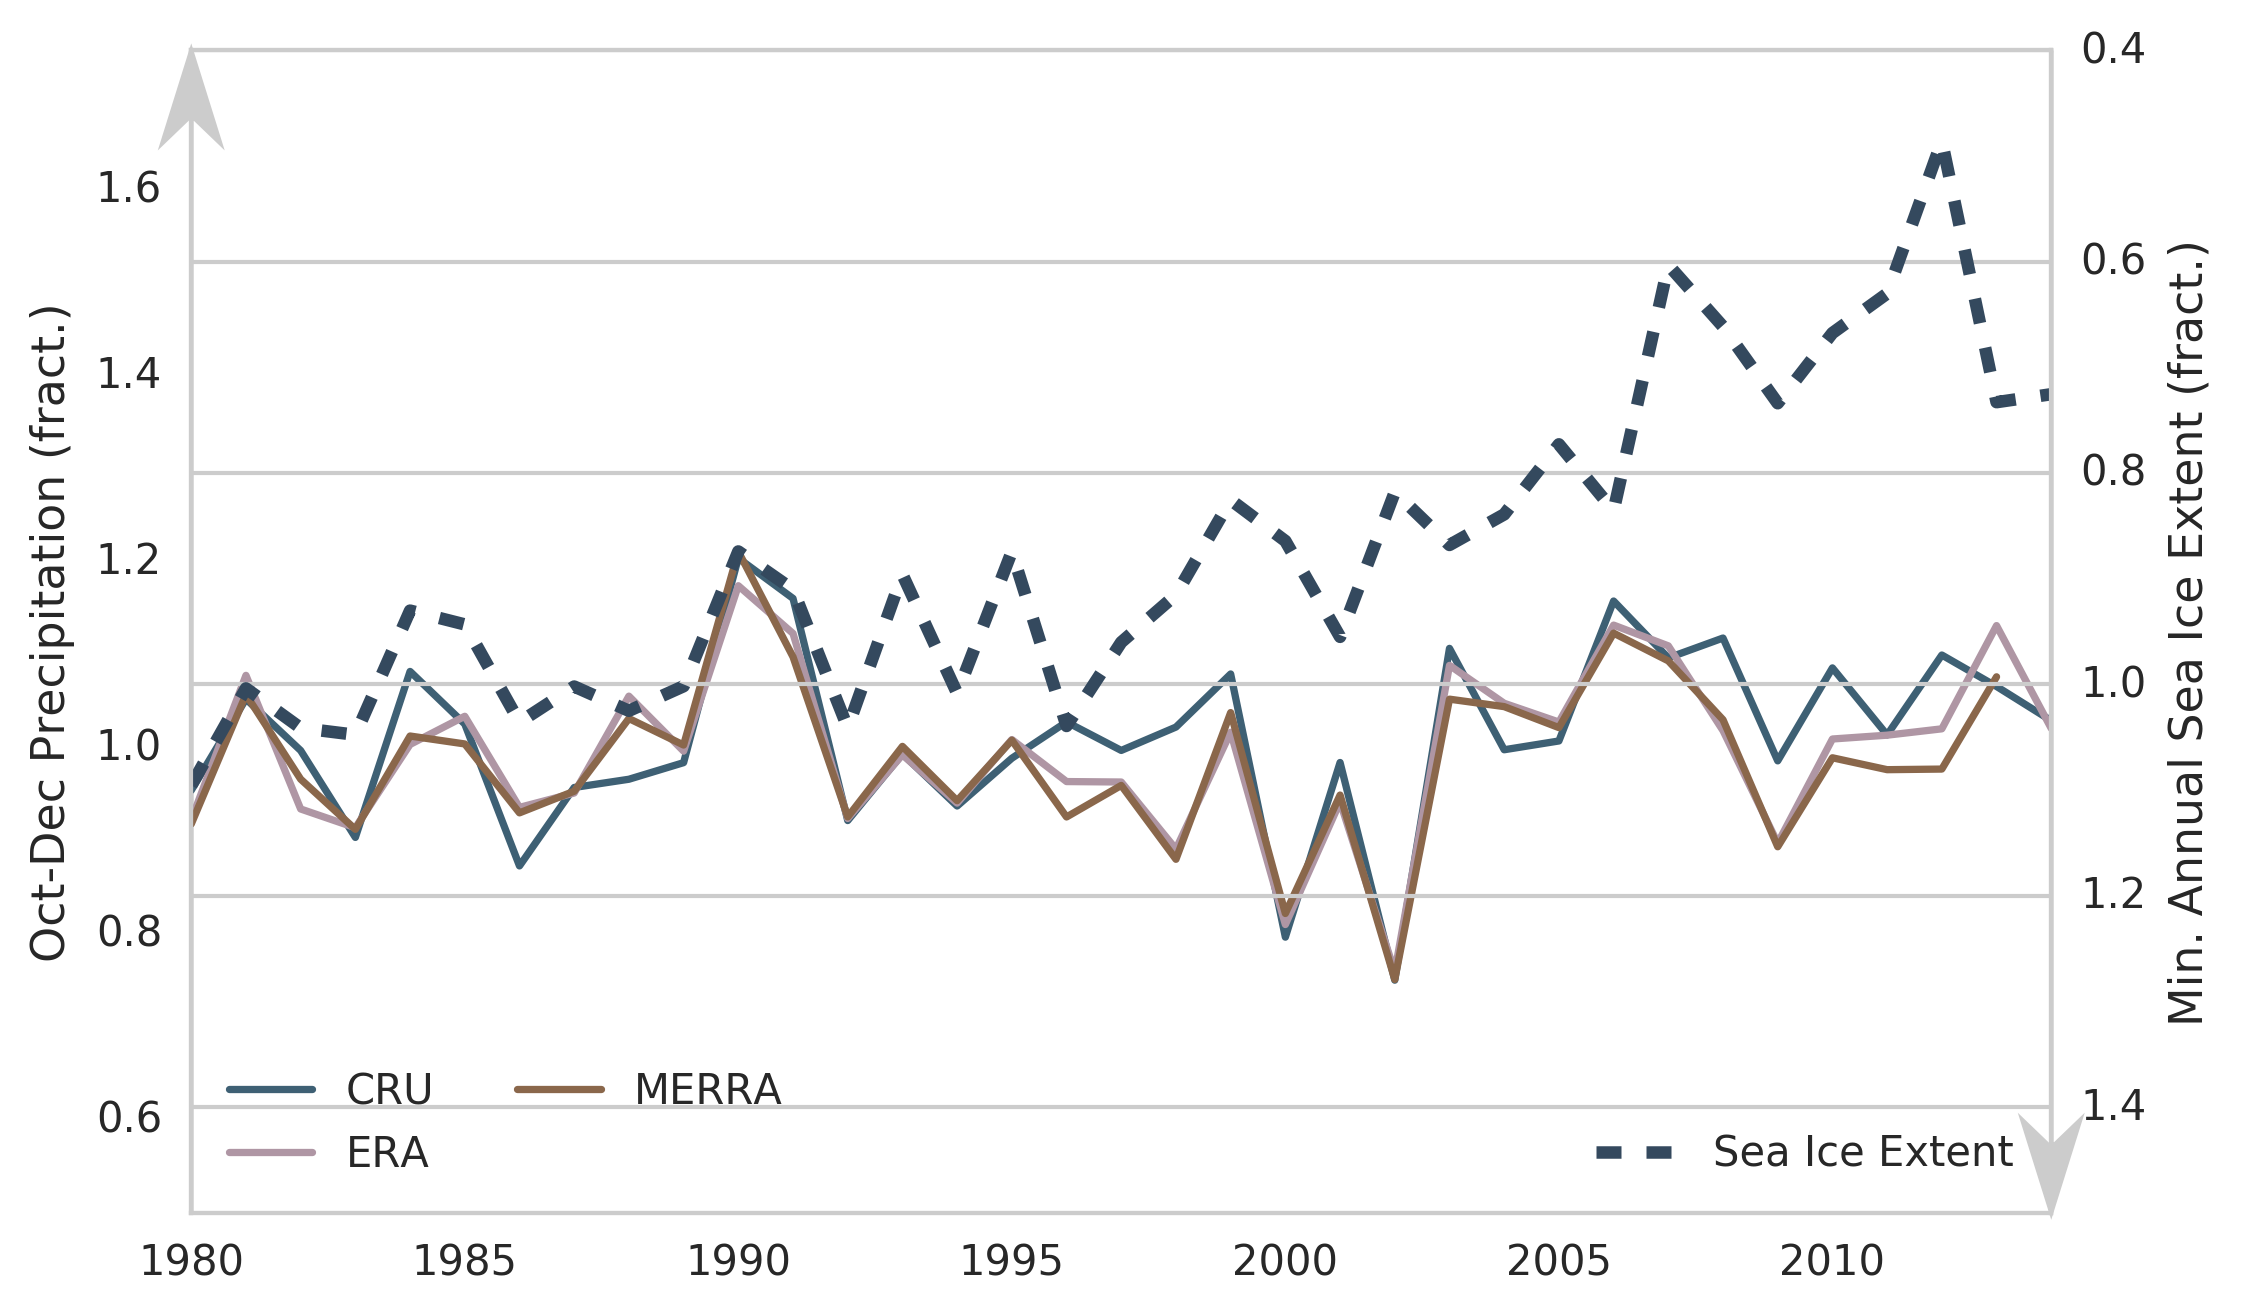
\includegraphics[width=12cm,keepaspectratio]{prec_seaice_ts}
  \caption{Timeseries (1980-2015) of fall precipitation (Oct - Nov) over the central Arctic drainage basin, (left axis) compared to minimum annual sea ice extent (right axis).}
  \label{fig:prec_ice_ts}
\end{figure}

% Motivation and establishing a connection between sea ice extent and precipitation
Our hypothesized relationship between precipitation and sea ice extent builds on the observed interannual covariance of precipitation and sea ice extent across the central Arctic drainage basin.
Here we define the central Arctic drainage basin as the land areas draining to the core sea ice regions of the Arctic ocean, including the Siberian Shelf (mainly the Kolyma and Lena Rivers) and Canadian coast (mainly the Mackenzie River).
In Figure \ref{fig:prec_ice_ts}, which presents the timeseries observed annual minimum sea ice extent and October-December precipitation from the MERRA and ERA-Interim reanlysis and CRU dataset.
Using the Spearman rank-order correlation measure, the MERRA, ERA, and CRU datasets exhibit correlations of -0.38, -0.40, and -0.52 respectively.
The observed relationship (e.g negative correlations) is most prominent prior to 2000.
This last point raises the question of whether or not the two processes were indeed related through a physical coupling that is limited by a threshold mechanism, or if these two processes are perhaps driven by a common forcing.

\begin{figure}
  \centering
  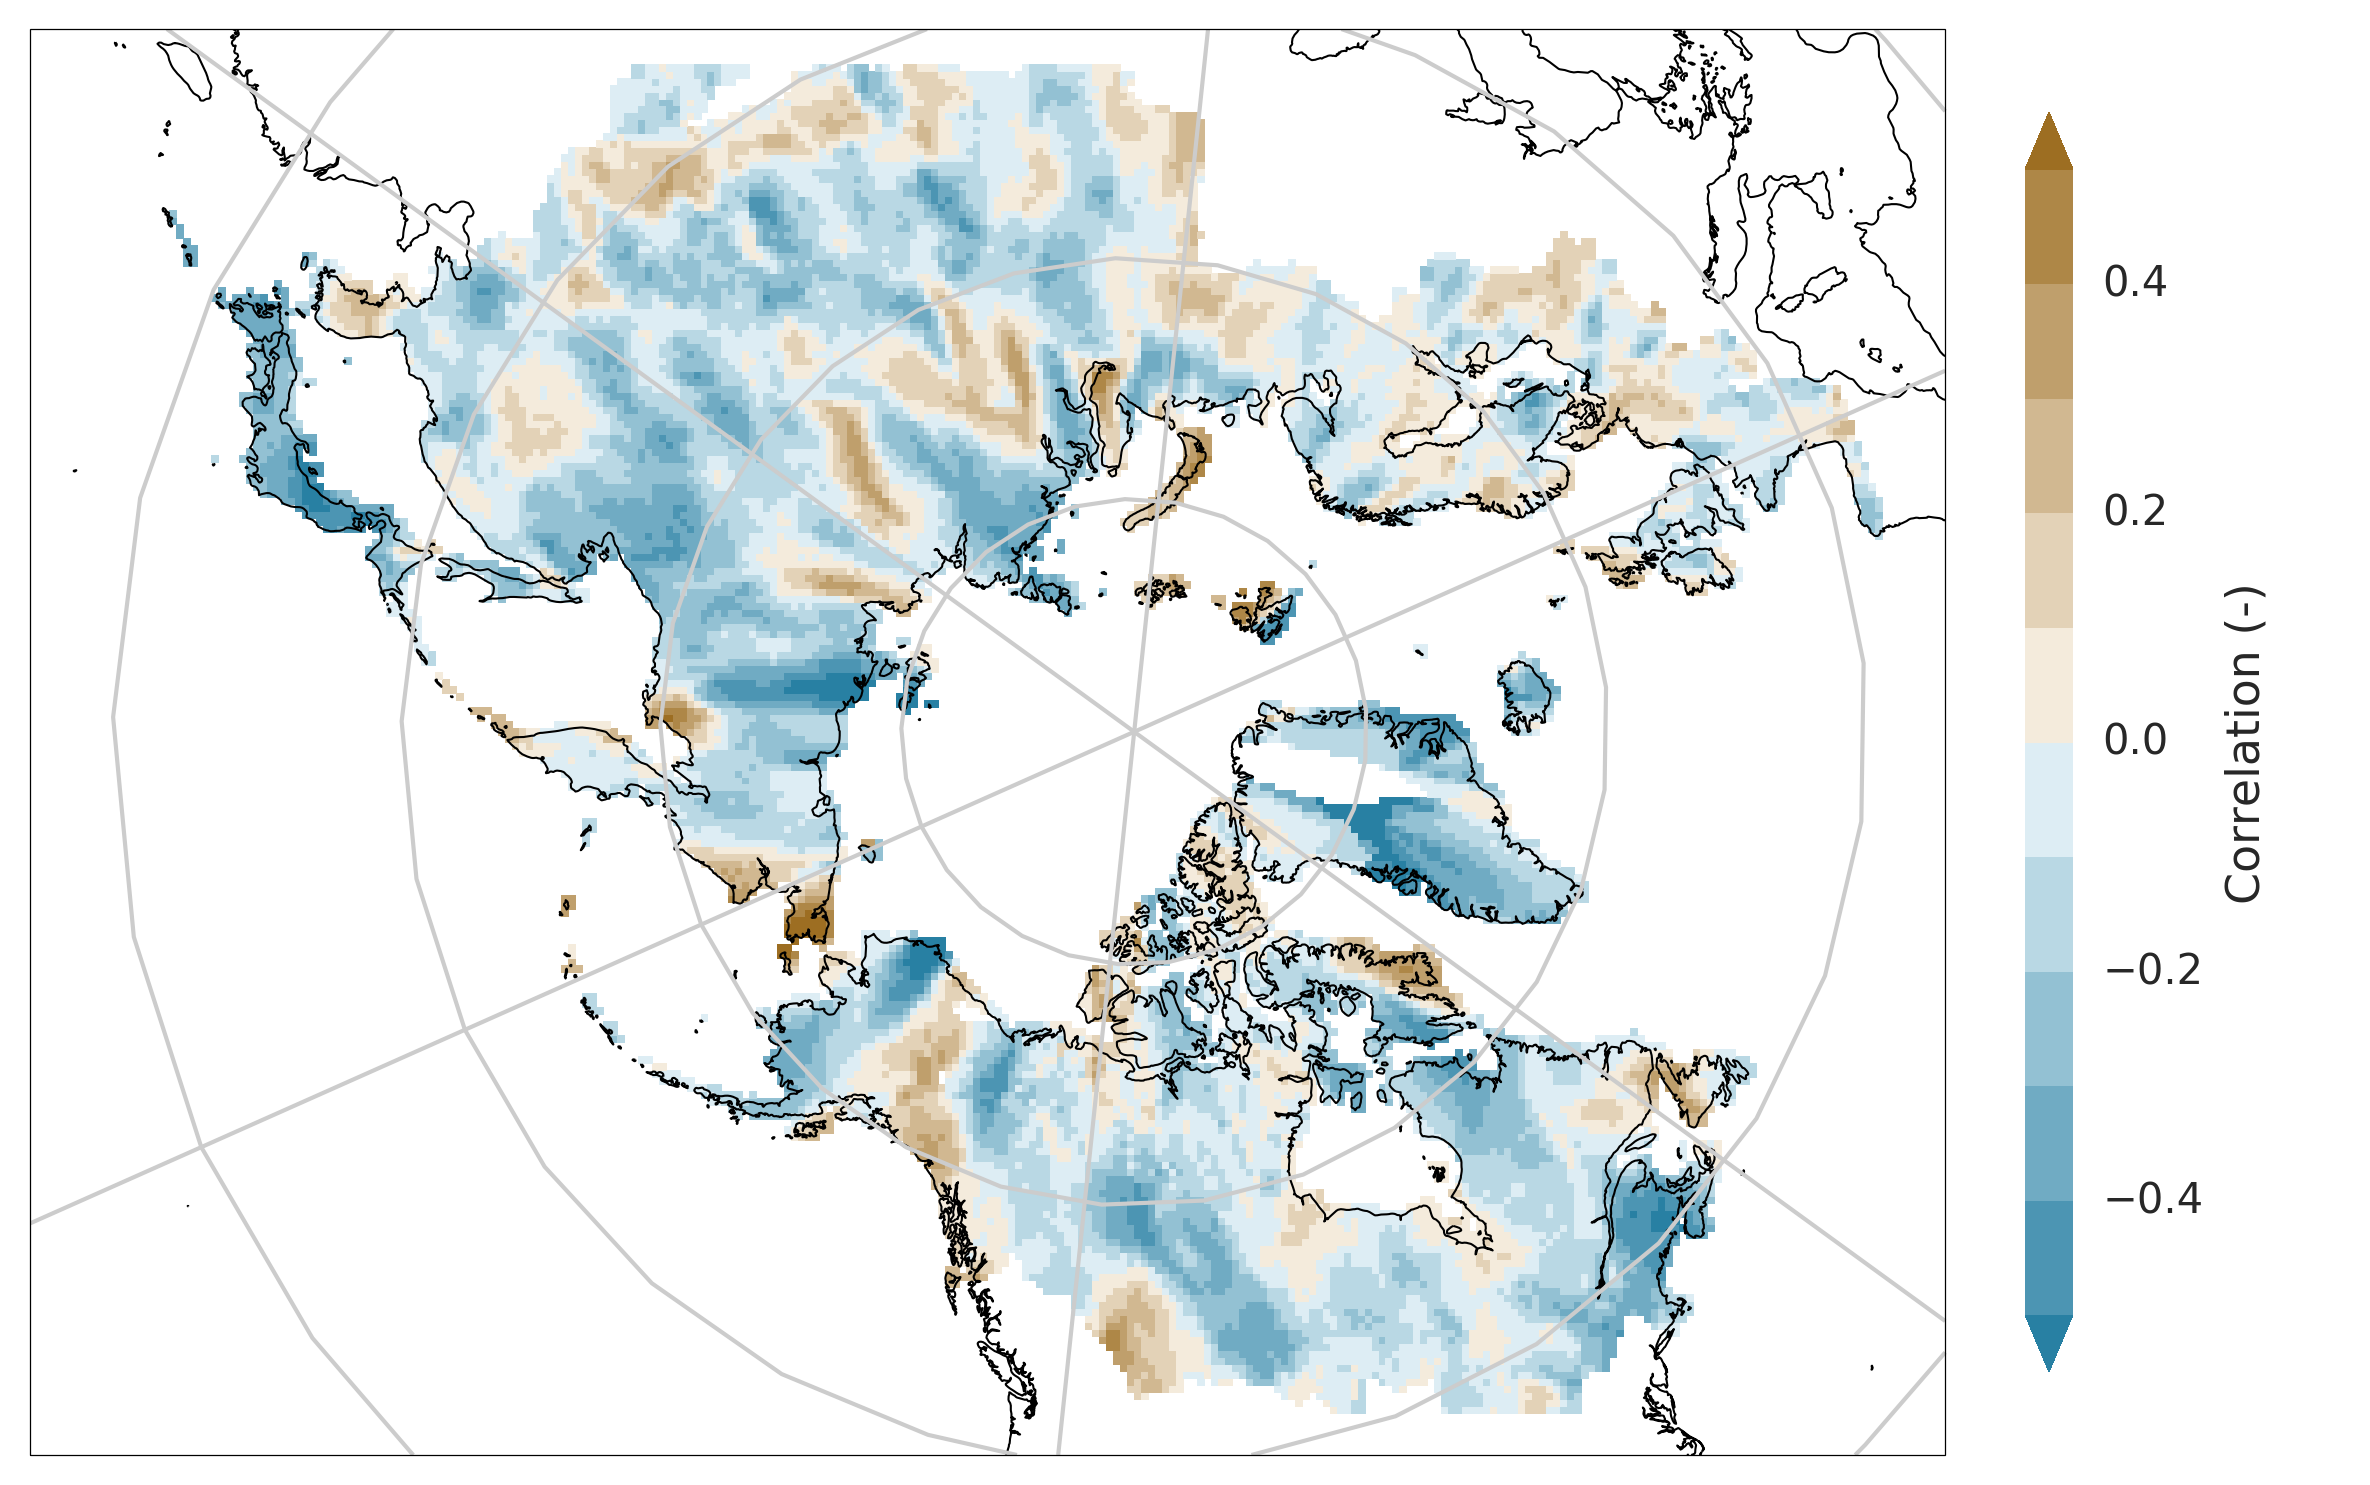
\includegraphics[width=12cm,keepaspectratio]{cru_correlation}
  \caption{Spearman rank-order correlation coefficients comparing observed minimum annual sea ice extent with gridded Oct-Dec precipitation from CRU. Time period 1980-2015.}
  \label{fig:prec_spatial_corr}
\end{figure}

The spatial pattern of correlations is somewhat more heterogeneous.
In Figure \ref{fig:prec_spatial_corr} we compute the Spearman rank-order correlation coefficients between October-December precipitation from the CRU dataset and minimum annual sea ice extent at each grid cell within the RASM domain.
Across most of the domain, the correlations are found to be below zero, with the most negative correlations occurring across Siberia and North America.
Correlations across Europe are predominantly near zero or positive.
From this analysis, we proceed knowing that there is a moderately consistent statistical relationship between sea ice extent and precipitation, especially in the high-latitude regions of the study domain.
In the following sections, we will attempt to understand the mechanisms driving this apparent relationship.

\subsection{RASM simulations}
% RASM sea ice sensitivity
We turn now to the distribution of sea ice extent in the three RASM simulations described in Section \ref{sec:data_models_ch5}.
Figure \ref{fig:sea_ice_box} shows box-and-whisker plots of sea ice extent from the three RASM simulations compared to the NSIDC observations.
Compared to $RASM_{CONTROL}$, $RASM_{RSI}$ and $RASM_{RSH}$ have mean fall season sea ice cover reductions of 3\% and 11\% respectively.
However, compared individual RASM simulations, the observations of sea ice extent demonstrate significantly more interannual variability.
In fact, individual months (e.g. October) have interannual standard deviations of 1.6 to 3.5 times smaller than the observations.
In section \ref{sec:soms}, we correct for this issue in our analysis by using the combination of these three simulations together.
We assert that the combined distribution of sea ice extents the RASM simulations adequately represents the range of observed sea ice extents during the fall season.

\begin{figure}
  \centering
  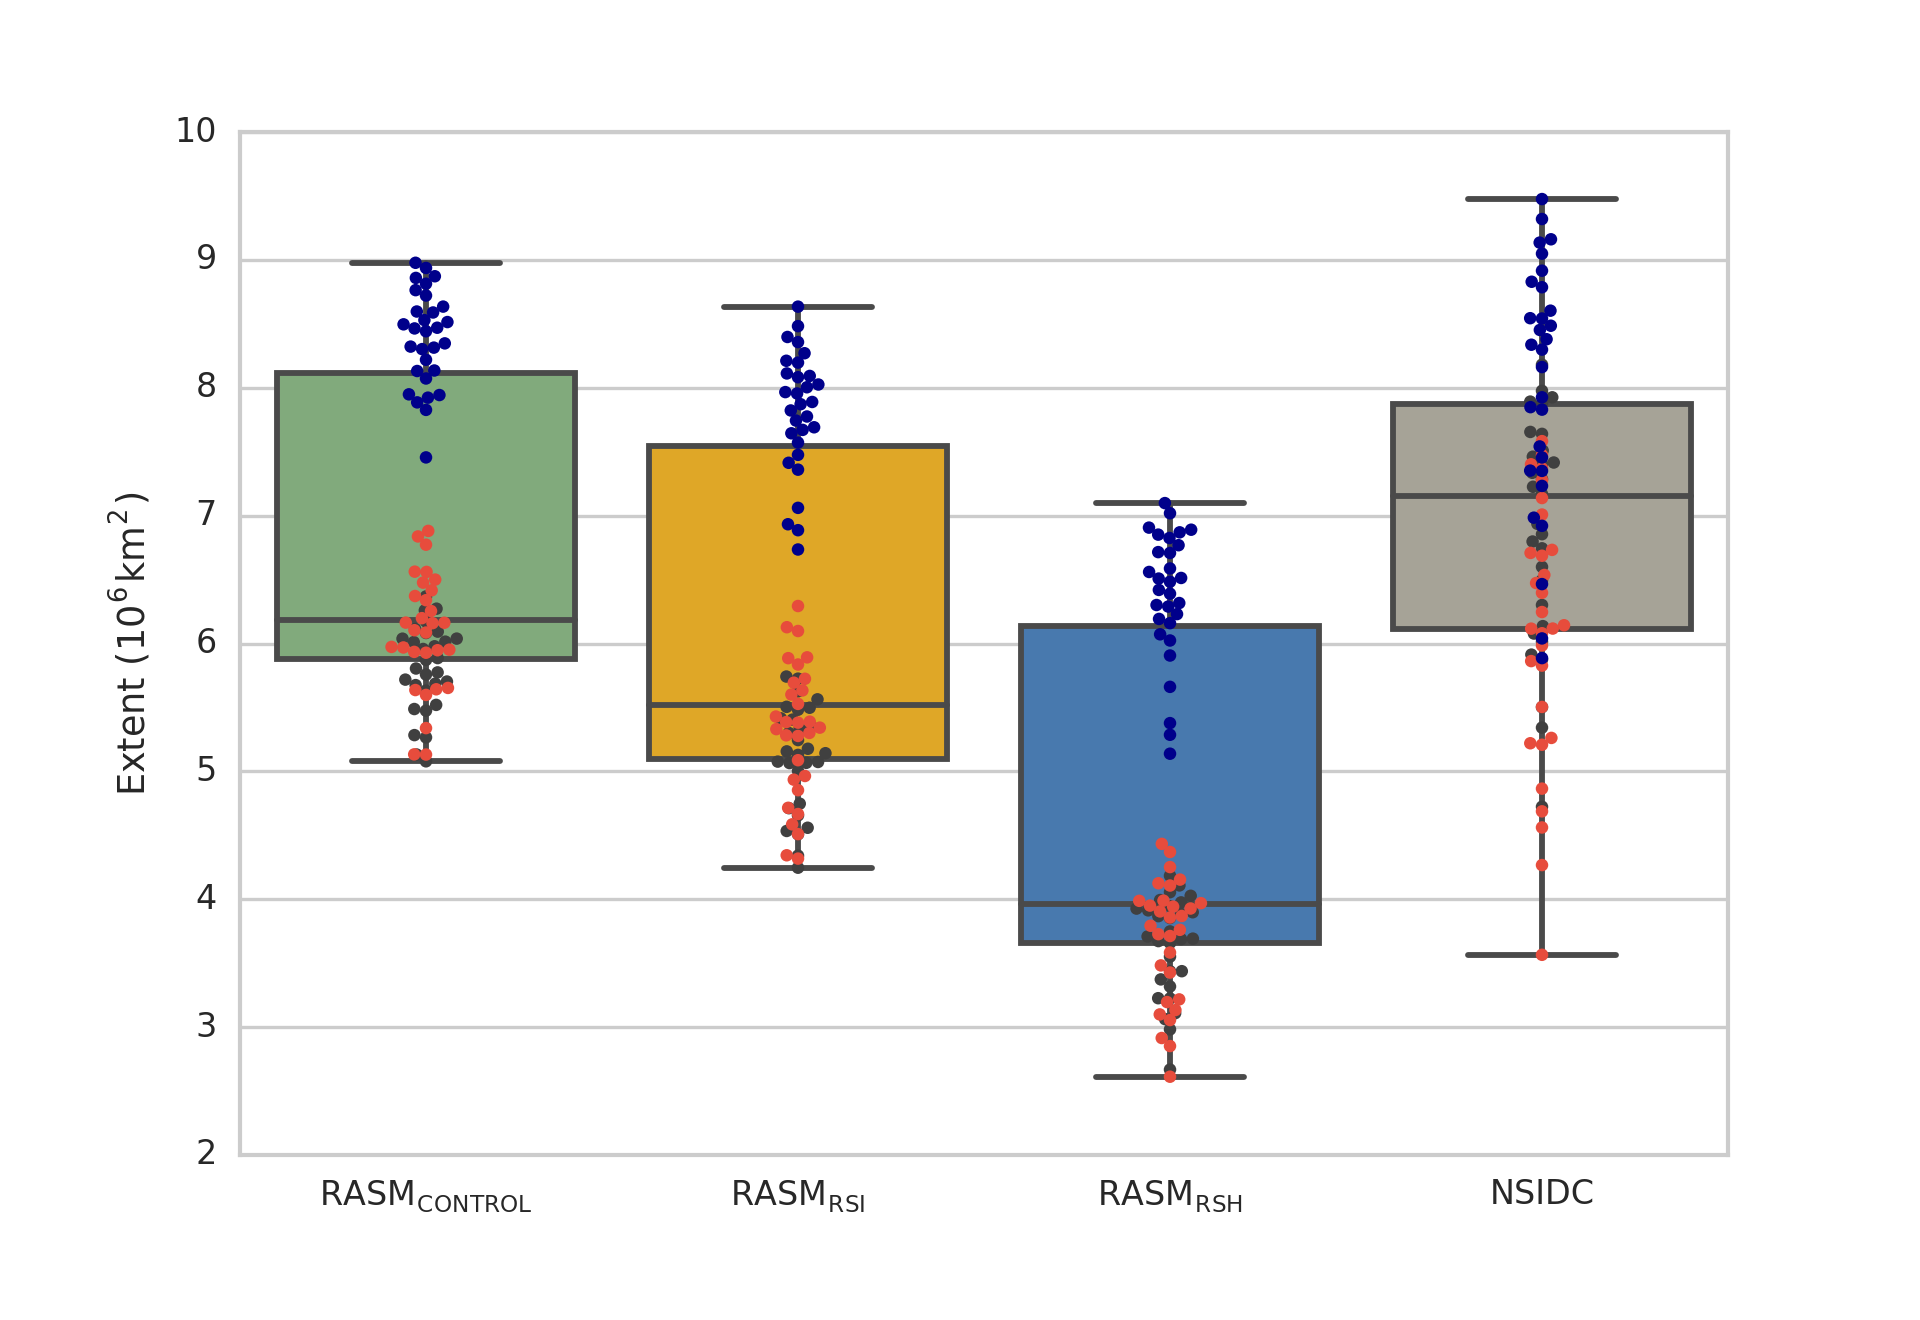
\includegraphics[width=12cm,keepaspectratio]{seaice_boxplots}
  \caption{Distribution of fall (Oct - Nov) sea ice extent in RASM and the NSIDC sea ice index. Time period 1985-2015.}
  \label{fig:sea_ice_box}
\end{figure}

% water budget changes
Figure \ref{fig:fwb} presents the freshwater budget for the three RASM simulations, summarized for the fall months (October-December).
The total moisture convergence for the three simulations are all within 0.05\% of one another.
The reductions in sea ice extent in $RASM_{RSI}$ and $RASM_{RSH}$, shown in Figure \ref{fig:sea_ice_box}, yield increases in evaporation from the ocean of 13\% and 52\%, respectively.
These changes in evaporation from the ocean translate to more modest increases in precipitation over the ocean of 3\% and 11\%.
Associated reductions in convergence over the ocean mask, defined here as P-E between October and December, are found to be 2\% and 10\%.
Finally, while precipitation over land is found to increase relative to the baseline case for both $RASM_{RSI}$ and $RASM_{RSH}$, the increases are relatively small (1\% and 3\% respectively).
Summarizing the water budget, we find that the forced decreases in $RASM_{RSI}$ and $RASM_{RSH}$ lead to significant increases in ocean evaporation but relatively small changes in precipitation over land, despite relatively large changes in ocean evaporation.
Changes in the spatial distribution of precipitation (not shown) lack a regional signal.
While this muted response may be partially explained by the limited interannual variability in the RASM sea ice extent, it also indicates that changes in evaporation from the Arctic Ocean will have to be accompanied with changes in circulation patterns if increases in precipitation are to be attributed to sea ice loss.

\begin{figure}
  \centering
  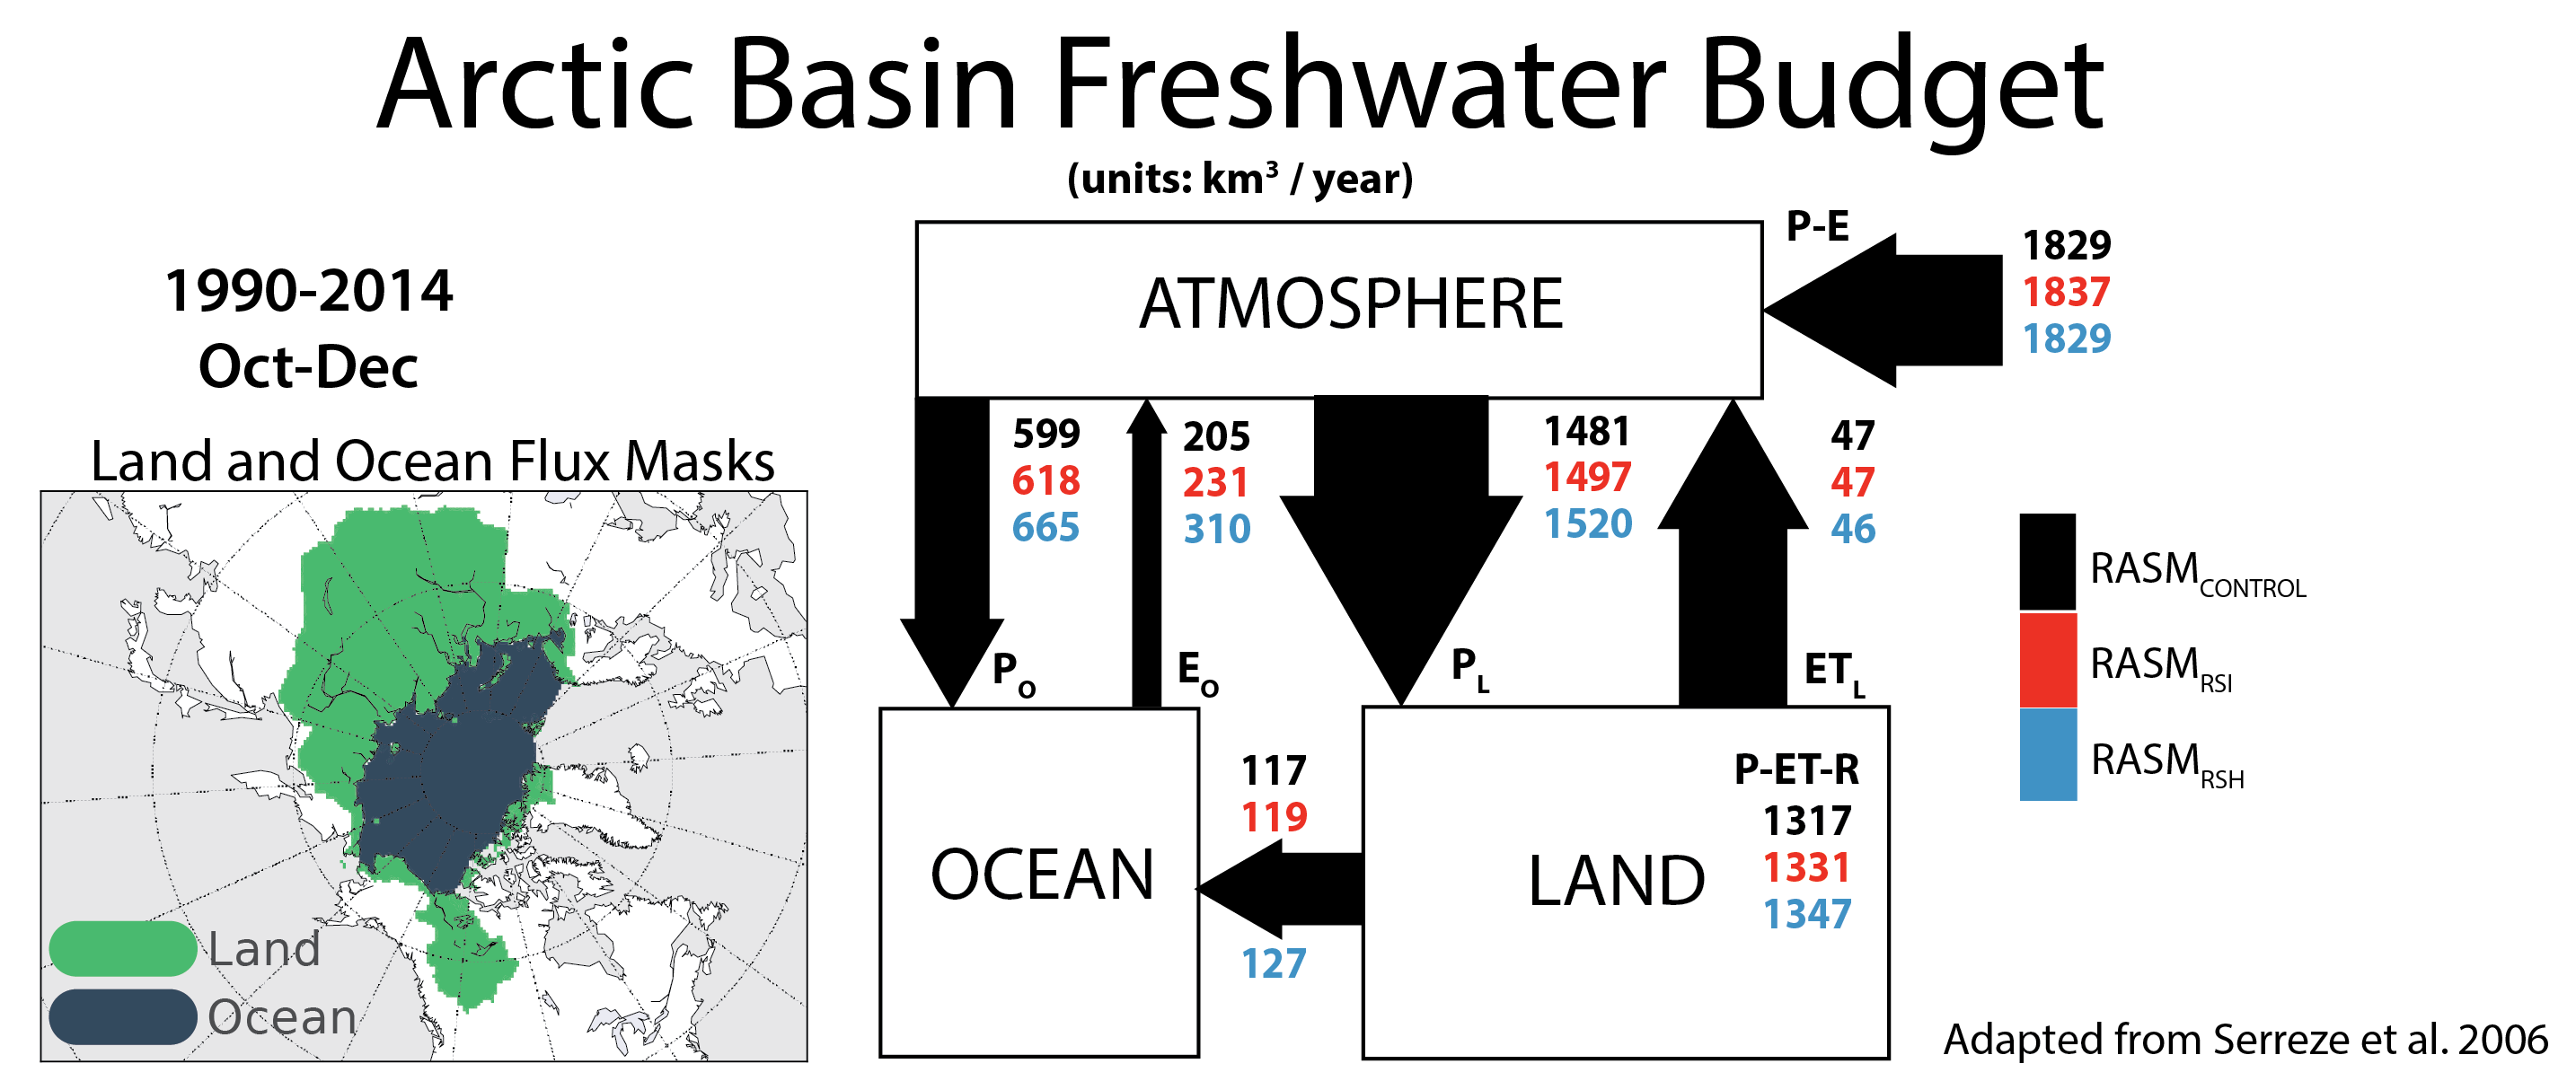
\includegraphics[width=14cm,keepaspectratio]{fresh_water_budget}
  \caption{Arctic freshwater budget, adapted from \citet{Serreze_2006a}.}
  \label{fig:fwb}
\end{figure}

\subsection{Self-Organizing Maps}
\label{sec:soms}
% SOM analysis
Given the relatively small sea ice sensitivity in the regional freshwater budget, we have applied the Self-Organizing Map \citep{Kohonen_1998,Hewitson_2002} technique on standardized evaporation anomalies across the Arctic Ocean.
The goal of this analysis was to provide insight into the coupling between ocean sourced evaporation and anomalies in precipitation over land during the fall season.
SOMs are useful technique for dimension reduction, allowing for the identification of unique climatological patterns.
They are are a type of unsupervised machine learning, utilizing artificial neural networks.
SOMs have been previously applied in studies of polar climatology to study synoptic scale atmospheric circulation \citep[e.g. ][]{Cassano_2007}, extreme weather events \citep[e.g. ][]{Cassano_2015,Glisan_2016}, and coupled ocean-atmosphere processes \citep[e.g. ][]{DuVivier_2016}.
In our analysis, we trained a 2x4 SOM, using standardized ocean evaporation anomalies north of 55$^{\circ}$ N. from each of the three RASM simulations described in Section \ref{sec:data_models_ch5} for fall months (October - December) between 1985 and 2014.
In total, the training dataset was comprised of 270 months of evaporation anomalies.
We used a evaluation metric of Euclidean distance, a learning rate of 0.001, and a maximum number of iterations of 2000.
The SOM was initialized with random fields from a standard normal distribution.
Further details on the SOM algorithm can be found in \citet{Reusch_2005} or \citet{Cassano_2015}.

% MASTER SOM
\begin{figure}
  \centering
  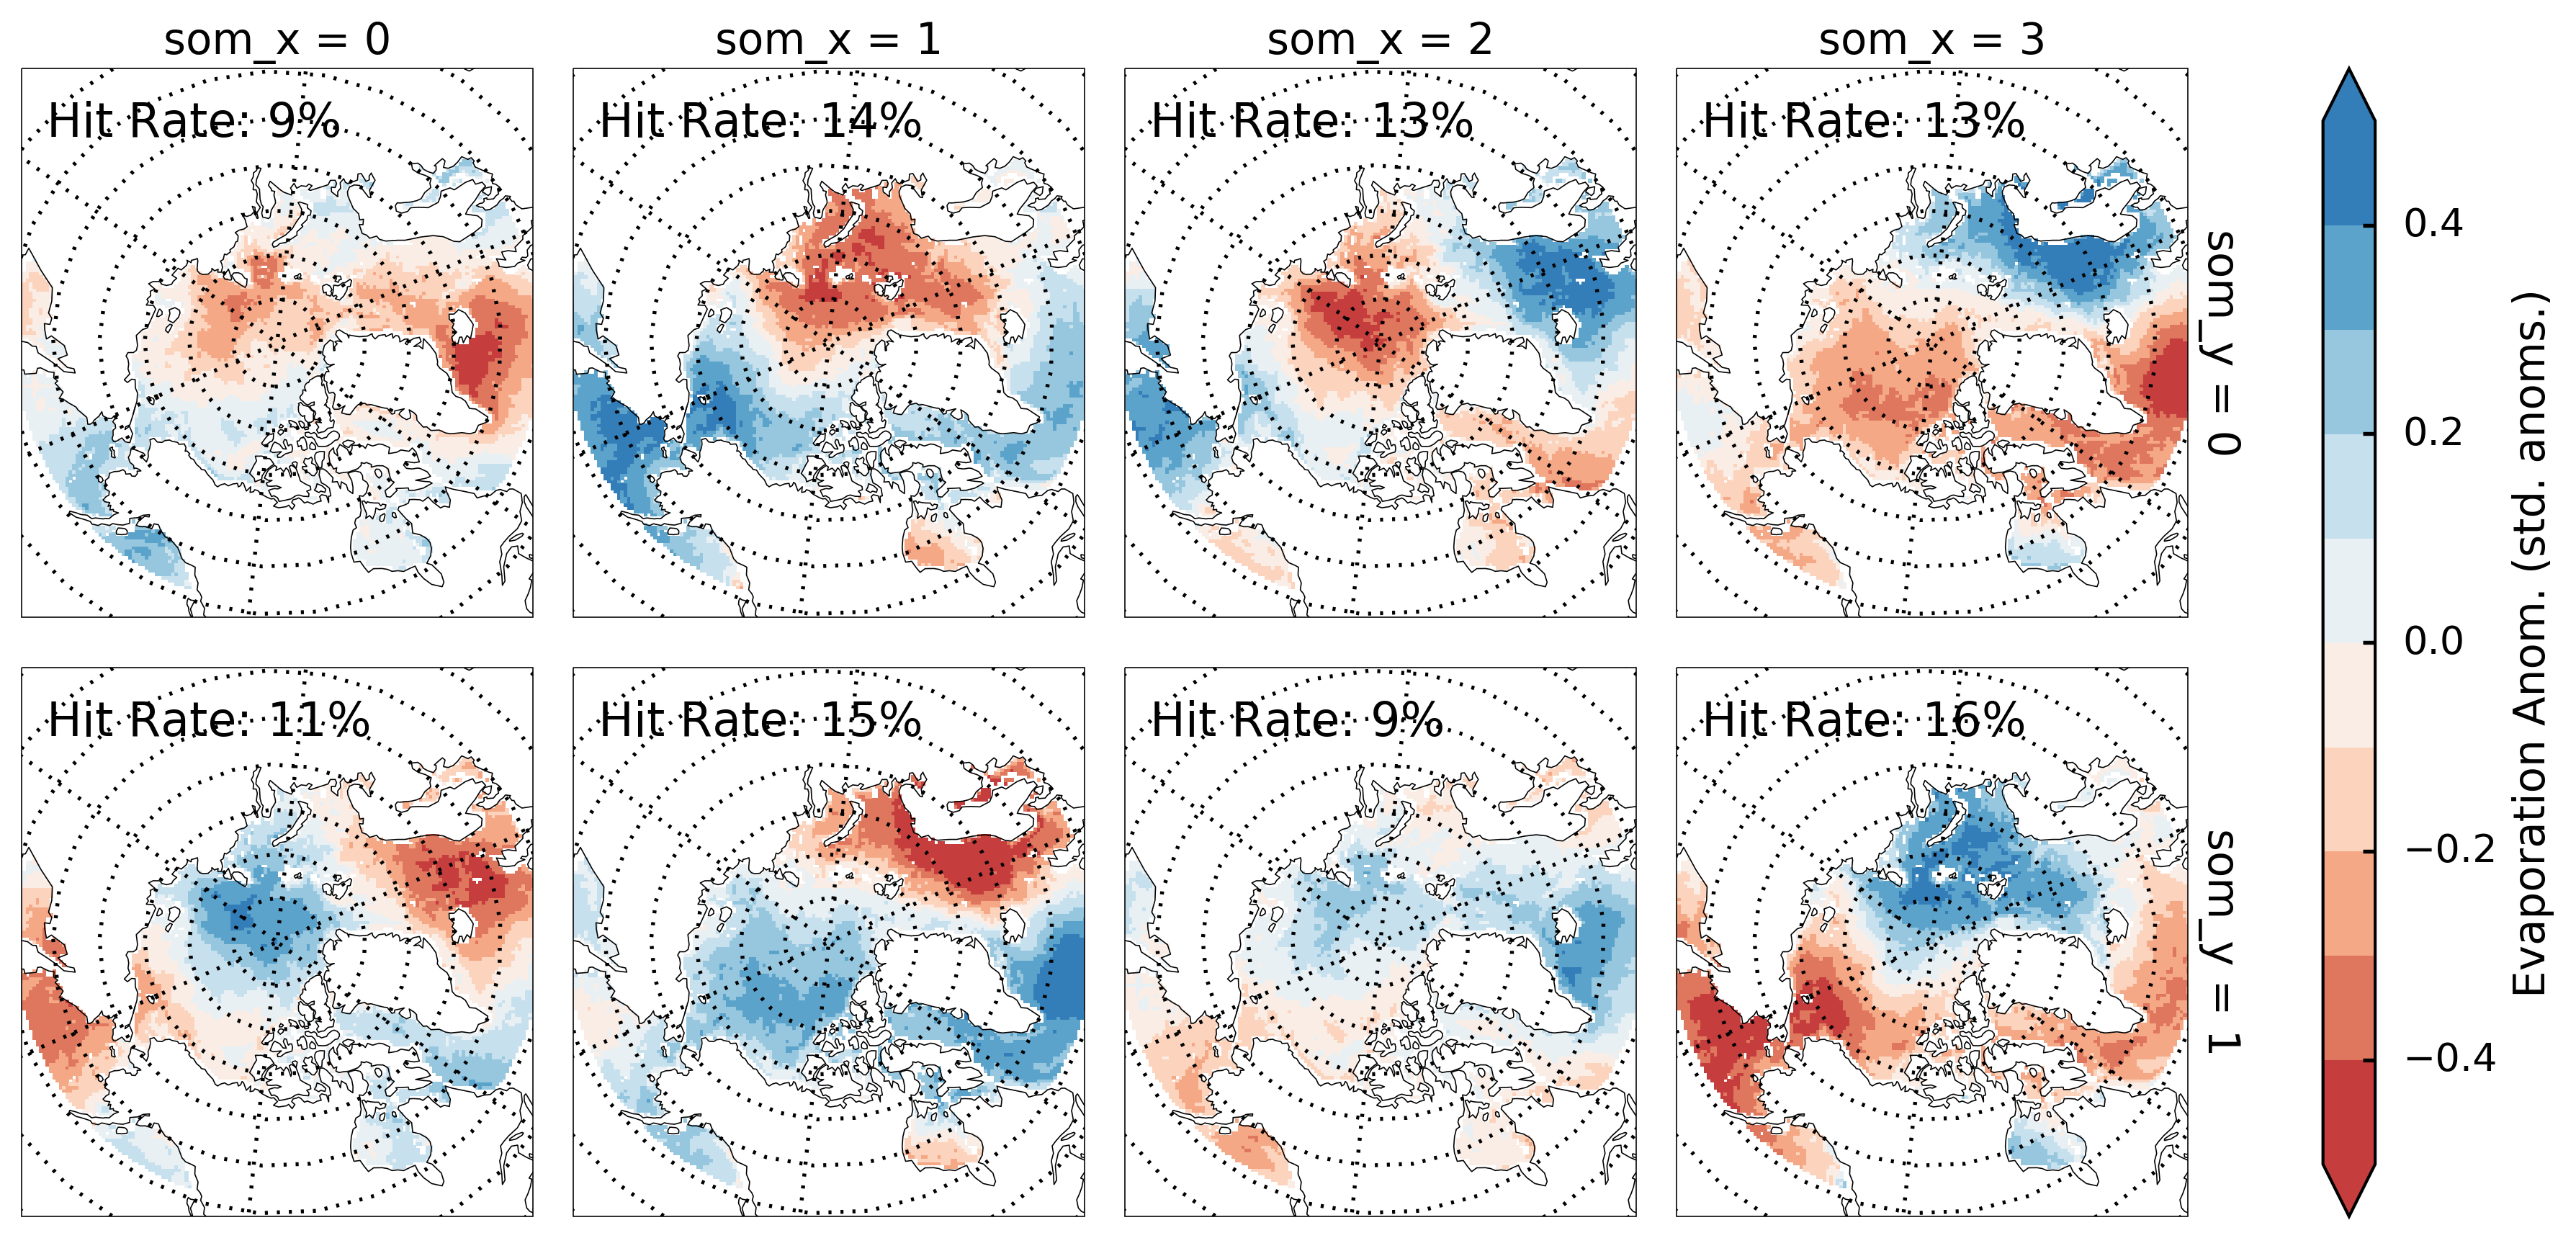
\includegraphics[width=14cm,keepaspectratio]{master_som}
  \caption{Master SOM. The hit frequency is shown in the top left corner.}
  \label{fig:master_som}
\end{figure}

The full trained Kohonen Layer (or Master SOM) is shown in Figure \ref{fig:master_som}.
The SOM algorithm identified characteristic spatial patterns of evaporation anomalies.
Here we will focus our analysis on four SOM nodes that exhibit the largest hit rate and evaporation patterns of interest: (0,1), (0,3), (1,0), and (1,2).
In terms of precipitation, we will show that the first two represent generally wet patterns while the second two represent generally dry patterns.
In each of these patterns, the combined position, sign, and magnitude of evaporation anomalies in the central Arctic, Kara/Barents sea, and North Atlantic Ocean are characteristically different.

% Composite SOM
\begin{figure}
  \centering
  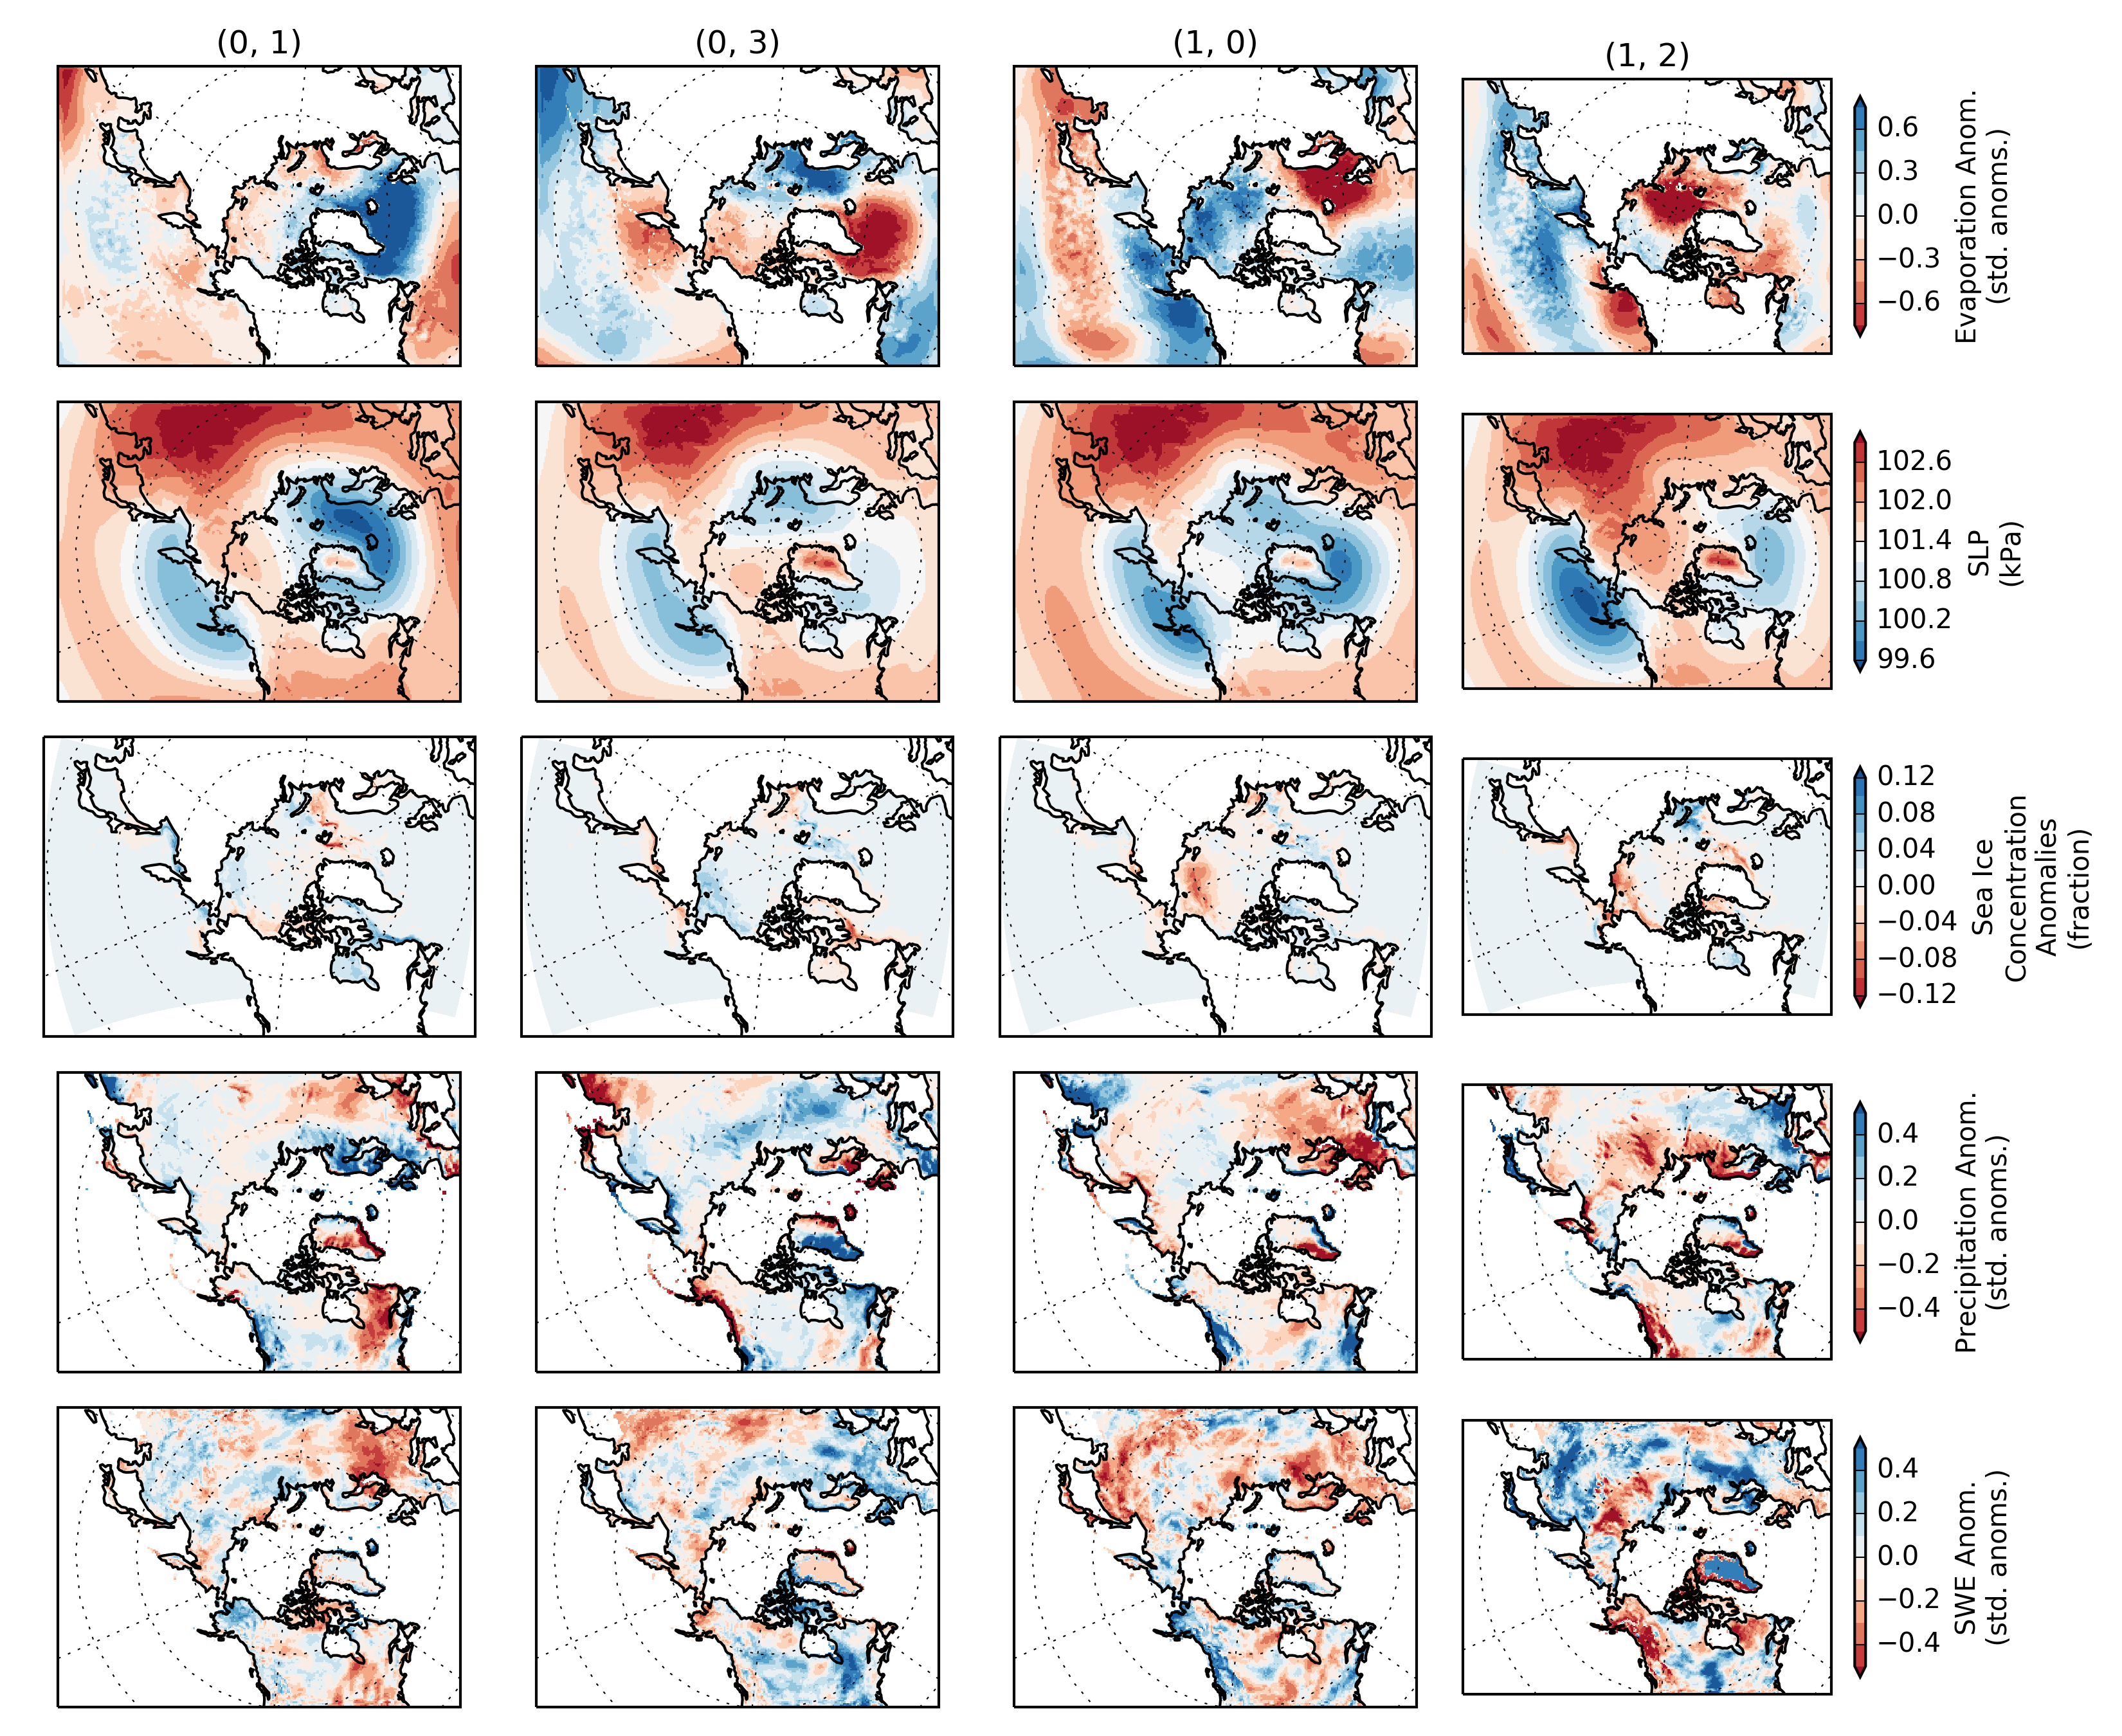
\includegraphics[width=15cm,keepaspectratio]{composite_som}
  \caption{SOM nodes (0,1), (0,3), (1,0), and (1,2) mapped to ocean evaporation, sea level pressure (SLP), sea ice concentration, precipitation over land, and snow water equivalent. Except for sea level pressure, values plotted are the average anomalies across all the members of each node.}
  \label{fig:composite_som}
\end{figure}
% TODO: get the subplots to align better

Figure \ref{fig:composite_som} presents the composite fields for the four SOM nodes discussed above.
Here we focus on ocean evaporation, sea level pressure (SLP), sea ice concentration, precipitation over land, and snow water equivalent.
For node (0,1), anomalously high evaporation rates from the North Atlantic are accompanied by anomalously low pressure in the region.
This combination is found to lead to positive precipitation anomalies over Northern Europe.
Node (0,3) exhibits positive evaporation anomalies in the Kara and Barents Seas and negative evaporation anomalies in the North Atlantic.
SLPs for this node are anomalously high across North America from Alaska to Greenland, indicating a southward shift of the storm track.
Corresponding precipitation anomalies for node (0,3) are positive over eastern Europe and central Siberia.
Neither of these nodes have substantial sea ice concentration anomalies that can be clearly tied to evaporation or precipitation anomalies.  % TODO: we may want to change how the anomalies in sea ice concentration are calculated so that this is more sensitive

The selected dry nodes, (1,0) and (1,2), are respectively characterized by large regions negative evaporation anomalies east and north of Greenland and positive anomalies in the central Arctic and Siberian Shelf.
Both nodes are mapped to negative sea ice concentration anomalies along the Siberian Shelf.
In node (1,2), positive sea ice concentration anomalies in the Kara Sea correspond to the negative anomalies ocean evaporation, although the spatial extent is considerable larger in the evaporation anomalies.
Node (1,2) also includes positive SLP anomalies across the central Arctic.

% Hit Map
\begin{figure}
  \centering
  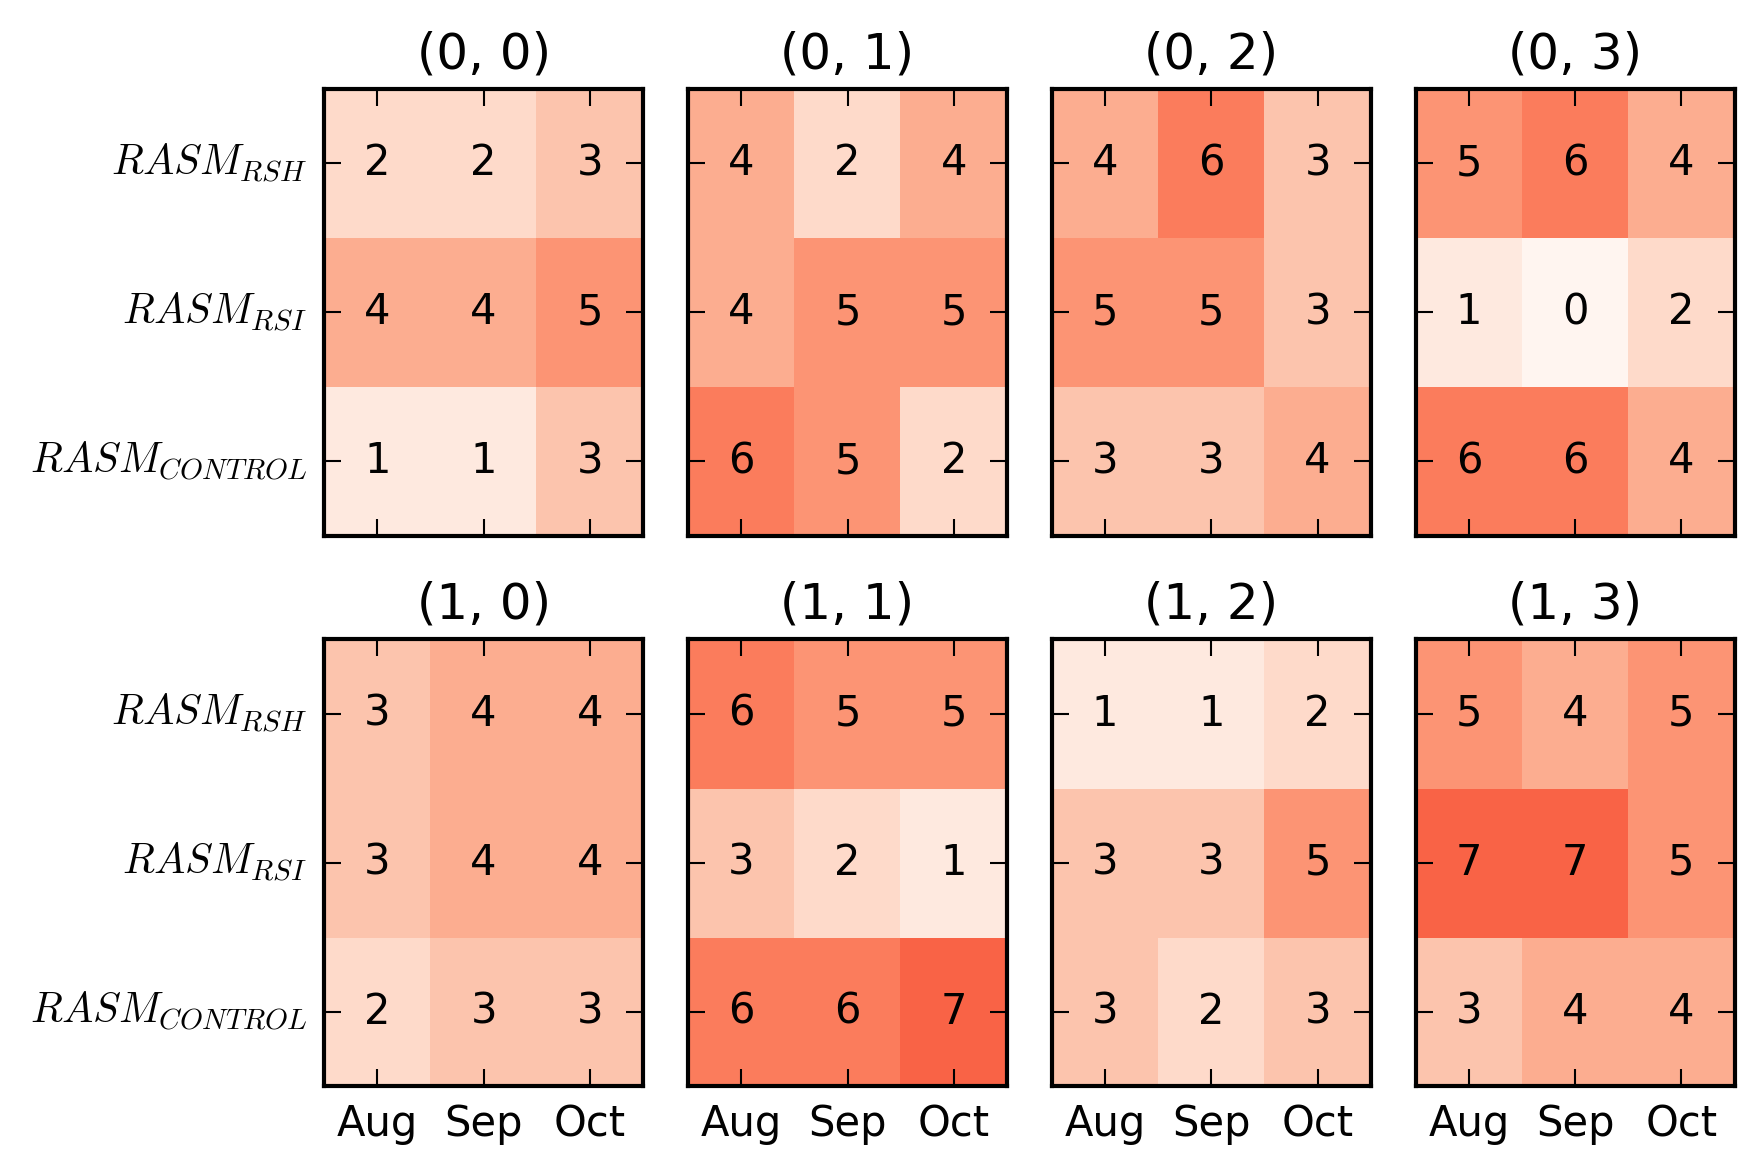
\includegraphics[width=10cm,keepaspectratio]{som_hit_freq}
  \caption{SOM hit frequency by month and RASM simulation.}
  \label{fig:som_hit_freq}
\end{figure}

The trained SOM can be used to identify the frequency of occurrence of each pattern as a function of month (October, November, or December) and RASM simulation ($RASM_{CONTROL}$, $RASM_{RSI}$, or $RASM_{RSH}$).
Figure \ref{fig:som_hit_freq} plots the mapping frequency, by month and simulation, for each node in the 2x4 SOM.
Node (0,1), which as we discussed above has a large region of positive evaporation anomalies across the North Atlantic, occurs nearly twice as frequently in $RASM_{RSH}$ as in $RASM_{CONTROL}$.
The opposite is found in node (0,3), where the hit frequency is found to decrease under reduced sea ice conditions.
Interestingly, the hit frequency for dry nodes [e.g. (1,0) and (1,2)] is mostly stable between the simulations.
On the whole, the SOM analysis may indicate that decreasing sea ice extent and the associated evaporation changes are most likely to contribute to wetting trends over land when these changes are accompanied by a shift in atmospheric circulation [e.g. node (0,3)].
In fact, global climate models tend to suggest that future Arctic climate will be stormier \citep{Vavrus_2012} and that winter circulation patters may trend toward a more variable pattern.
However, the fact that the patterns with large shifts in frequency [(0,1) and (1,2)] shift in directions that limit the impact of sea ice loss, indicates that the precipitation response may be dampened.

\section{Conclusions}
\label{sec:conclusions_ch5}

In summary, we have investigated the relationship between sea ice extent and early winter precipitation over the Pan Arctic land masses.
We have demonstrated observed interannual covariance between sea ice extent and precipitation over land, and identified a break in the presumed relations circa year 2000, about the minimum annual sea ice extent began to decline most rapidly.
A simple water budget analysis highlighted that although relatively large changes in winter evaporation from the Arctic Ocean are expected (50\% in our lowest sea ice simulation), these changes are proportionally small when compared to the precipitation flux over land.
Furthermore, the modest increases in terrestrial fall season precipitation predicted by RASM under reduced sea ice conditions indicate there will have to be significant circulation changes in the future if ocean sourced evaporation is likely to significantly impact precipitation over land.
Our SOM analysis has also pointed us in this direction, which is that the ties between evaporation and precipitation are only robust under certain atmospheric circulations.
Across Eurasia, the dominant coupling between precipitation and Arctic Ocean evaporation requires low pressure anomalies over the central Arctic, similar to the negative phase of the Arctic Oscillation \citep{Thompson_1998}.

Of particular interest is the sea ice state in the Kara and Barents Seas.
As sea ice declines, we expect that this coupling will become stronger, especially if the Arctic is to become stormier.
We have found that sea ice retreat along the Siberian shelf and north Alaskan coast is holds less influence on precipitation regional patterns.
In these areas, the circulation patterns (low pressure in North Pacific) tend to limit the influence of enhanced evaporation along the ice edge.
